\indent 実験3では, 認証機構の処理能力(計算効率)を評価するための実験を行った. 
不正ノードの存在しない環境でノード数を37, 74, 112, 148, 185に設定して
250回ずつシミュレーションを行い, それぞれの実行にかかった時間を調べた.\\
\indent 実験の結果は以下の通りである. \\

\begin{figure}
  \centering
  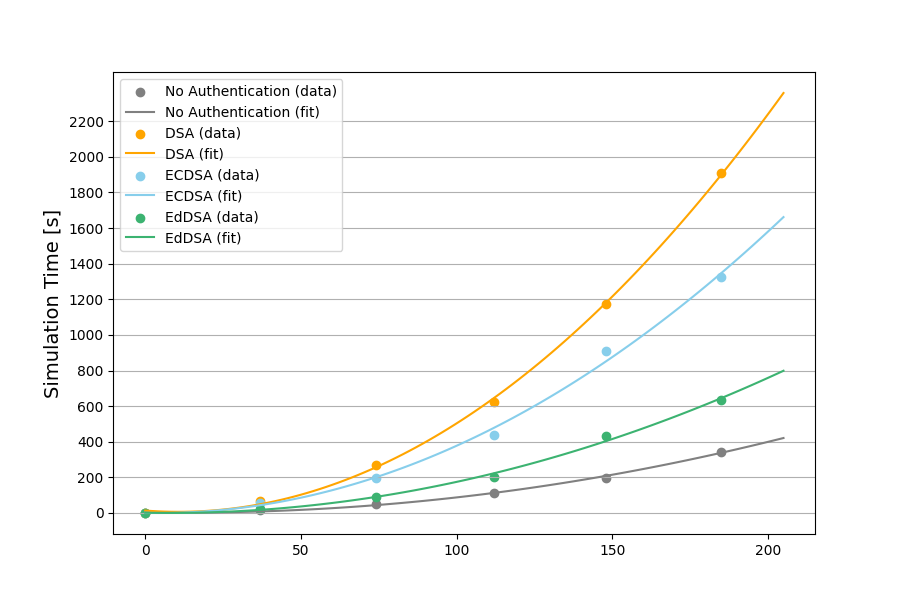
\includegraphics[width=1\textwidth]{figures/exp3_simtime.png}
  \caption{ノード数によるシミュレーション実行時間の変化}
  \label{fig:exp3_simtime}
\end{figure}

\setlength{\tabcolsep}{4pt}
\begin{longtable}{
    >{\raggedright\arraybackslash}p{3cm}
    >{\raggedright\arraybackslash}p{3.7cm}
    >{\raggedright\arraybackslash}p{2.5cm}
    >{\raggedright\arraybackslash}p{2.5cm}
    >{\raggedright\arraybackslash}p{2.5cm}
  }
  \caption{ノード数によるシミュレーション実行時間}
  \label{tab:exp3_simtime} \\
  \endfirsthead
  \hline
  % \multicolumn{1}{c}{Number of nodes} &
  % \multicolumn{1}{c}{No Authentication [s]} &
  % \multicolumn{1}{c}{DSA [s]} &
  % \multicolumn{1}{c}{ECDSA [s]} &
  % \multicolumn{1}{c}{Ed25519 [s]} \\ \hline \hline
  Number of nodes & No Authentication $[s]$ & DSA $[s]$ & ECDSA $[s]$ & Ed25519 $[s]$ \\ \hline \hline
  \multicolumn{1}{c}{$37$} &
  \multicolumn{1}{c}{$14.1802$} &
  \multicolumn{1}{l}{$69.9882$} &
  \multicolumn{1}{l}{$55.0108$} &
  \multicolumn{1}{l}{$24.4069$} \\
  \multicolumn{1}{c}{$74$} &
  \multicolumn{1}{c}{$50.5984$} &
  \multicolumn{1}{l}{$267.433$} &
  \multicolumn{1}{l}{$194.408$} &
  \multicolumn{1}{l}{$89.2728$} \\
  \multicolumn{1}{c}{$112$} &
  \multicolumn{1}{c}{$110.405$} &
  \multicolumn{1}{l}{$625.504$} &
  \multicolumn{1}{l}{$436.926$} &
  \multicolumn{1}{l}{$200.901$} \\
  \multicolumn{1}{c}{$148$} &
  \multicolumn{1}{c}{$196.971$} &
  \multicolumn{1}{l}{$1172.57$} &
  \multicolumn{1}{l}{$910.373$} &
  \multicolumn{1}{l}{$431.346$} \\
  \multicolumn{1}{c}{$185$} &
  \multicolumn{1}{c}{$345.059$} &
  \multicolumn{1}{l}{$1908.7$} &
  \multicolumn{1}{l}{$1324.55$} &
  \multicolumn{1}{l}{$635.155$} \\ \hline

  % $37$ & $14.1802$ & $69.9882$ & $55.0108$ & $24.4069$ \\
  % $74$ & $50.5984$ & $267.433$ & $194.408$ & $89.2728$ \\
  % $112$ & $110.405$ & $625.504$ & $436.926$ & $200.901$ \\
  % $148$ & $196.971$ & $1172.57$ & $910.373$ & $431.346$ \\
  % $185$ & $345.059$ & $1908.7$ & $1324.55$ & $635.155$ \\ \hline
\end{longtable}

\begin{longtable}{ccc}
  \caption{1回の署名作成と署名検証にかかった時間}
  \label{tab:exp3_sigtime} \\
  \endfirsthead
  \hline
  \multicolumn{1}{c}{プロトコル} &
  \multicolumn{1}{c}{署名作成時間 $[\mu s]$} &
  \multicolumn{1}{c}{署名検証時間 $[\mu s]$} \\ \hline \hline
  ECDSA & $371.020$ & $336.938$ \\
  Ed25519 & $31.349$ & $97.036$ \\ \hline
\end{longtable}

\indent 図\ref{fig:exp3_simtime}はシミュレーションパターンごとのノード数による
実行時間の変化を近似してグラフ化したものを, 表\ref{tab:exp3_simtime}はその具体的な
値を示したものである. さらに, 表\ref{tab:exp3_sigtime}にはECDSAとEdDSAにおいて, 1回の署名作成と
署名検証にかかった時間を示した. \\
\indent 図\ref{fig:exp3_simtime}, 表\ref{tab:exp3_sigtime}より, 
EdDSA, ECDSA, DSAの順番で実行時間が短いのがわかる. また, 
表\ref{tab:exp3_sigtime}に示すように, EdDSAがECDSAに比べて
署名生成, 署名検証にかかる時間が短いことから, EdDSAは
3つの署名方式の中で最も計算効率が良いということが確かめられた. 
さらに, ECDSAとEdDSAの計算効率の差はノード数が増加するほど, 
実行時間全体に与える影響が大きなっており, EdDSAが
よりスケーラビリティに優れていることを示唆している. 